\chapter{Binary Rewriting}
\label{binary_rewriting}

Binary rewriting is a software technique that transforms an executable by maintaining its original behaviour, while improving it in one or more aspects such as runtime performance, security and reliability. The research literature is full of examples of binary-rewriting methods applied to a variety of topics, including optimization \cite{Romer97instrumentationand}, code instrumentation \cite{PEBIL, BIRD}, security enhancements \cite{vx32}, software caching \cite{Valgrind, DynamoRio} and emulation \cite{Qemu}. Consequent to the advantages of binary rewriting, numerous binary rewriters have been developed. Typically they fall into two main categories \emph{static rewriters} and \emph{dynamic rewriters}, which can be further subdivided according the approach taken in the rewriting process, \emph{full rewriting} where the entire binary is rewritten and \emph{selective rewriting} where only relevant instructions are modified. 
\begin{description}

\item[Static binary rewriters] modify the executable file off-line allowing them to perform complex analysis and transformations. Due to their offline nature, \emph{relocation information} is required to identify code regions and address locations. The identification of code regions is necessary to ensure a full disassembly of the binary file. Disassembling  the entire code segment is an insufficient solution, as  compilers often insert data within the code segment (such as jump tables and padding). The identification of address locations is required to adjust addresses during the relocation phase. The necessity of relocate information can be avoided using a selective binary-rewriting approach \cite{BIRD, seccompsandbox} as the original code remains the same to the greatest extent possible. However, this approach allows only minimal transformations such as insertion of a trampoline instruction to jump into an instrumentation block and peephole optimizations. \footnote{A peephole optimization is an optimisation performed over a small set of instructions. It works by recognising sets of instructions that can be replaced by shorter or faster set of instructions.}

\item[Dynamic binary rewriters] modify the executable during its execution. The key advantage of this methods is that it does not require any relocation or symbolic information as at runtime the identification of the code regions and the address locations is straightforward. Unfortunately, dynamic rewriters introduce a significant overhead during execution, as all rewriting operations occur at runtime. This makes it infeasible to use a binary rewriter to perform complex transformation such as automatic parallelization as the overhead introduced is prohibitive. Consequent to this limitation, dynamic binary rewriters have been only employed for simply code instrumentation, and even in this case the overhead introduced is significant, for DinamoRIO 20\% and PIN 54\% as reported in \cite{Strata}. 
\end{description}

Despite their limitations, both static rewriting and dynamic rewriting can be successfully used to intercept system calls. In this section we focus on ELF\footnote{Executable and Linkable Format (ELF, formerly called Extensible Linking Format) is a common standard file format for executables, object code, shared libraries, and core dumps.} binary files that run on the Linux platforms, including both x86\_32 and x64 architectures. Several instrumentation tools have been implemented \cite{PEBIL, BIRD, REINS}, but none of them has been exclusively designed for intercepting system calls, though they can be used for accomplishing such a task. 

A system call interceptor based on binary rewriting, works by placing a branch instruction at each system call invocation within the application code to transfer control to the instrumentation code. As in the case of previous interceptor mechanisms, a way to pre and post process a system call invocation needs to be provided. This is accomplished by the instrumentation code, which executes a pre-routine, the system call and a post-routine in sequence, and then returns control to the application. A routine must be designed in such way to ensure that the program state is preserved across its execution, for example saving the state registers in the stack before their execution and restoring their values afterwards. This guarantees that the behaviour of the modified binary is the same as the behaviour of the original file.  In addition, this system call interceptor must be able to identify all instructions that issue a request for a system call. Linux provides three different ways to invoke a system call:

\begin{description}

\item[Interrupts] have been used by Linux to implement system calls on all x86 platforms since its first release. To execute a system call, a user process can copy the desired system call number to the \ci{EAX} register ( both x86\_32 and x64) and execute the instruction \ci{int 0x80}. This generates the interrupt 0x80 and the corresponding interrupt service routine is called. The task of this routine is to save the current state and call the appropriate system call handler based on the value of the \ci{EAX} register.Further information regarding the implementation of this routine can be found in the \emph{entry.S} file in the source of the kernel. However, this mechanism has turned out to be really slow since Pentium IV architectures, arising the need of a new efficient way to make system call. 


\begin{center}
\lstset{escapechar=@,style=asm}
\begin{lstlisting}[label=list:int,caption=Write system call invocation via interrupt on x86\_32 architecture]
  											     movl    $len,%edx       
  							  					 movl    $msg,%ecx       
       				 							 movl    $1,%ebx        
       				 			 				 movl    $4,%eax         
      							 				 int 	   $0x80
\end{lstlisting}
\end{center}




\item[Sysenter/Sysexit] instructions were introduced by Intel from the Pentium II and later CPUs to fix the overhead issue correlated to the use of interrupts as mechanism to invoke system calls. \lstinline$SYSENTER$ can be executed by any application, while  \lstinline$SYSRET$ can only be executed by ring 0 programs.These instructions are used as a fast way to transfer control from user mode (ring 3) to privileged mode (ring 0) and back quickly, allowing a fast and safe way to execute system routines from user mode.These instructions directly rely on the \textit{Model Specific Registers} (MSR) \cite{Intel} which complicates that way to invoke a system call for an user. Instead of using this mechanism directly, it is strongly recommended to use the system call entry/exit point exported in user space by the kernel since version 2.6 as presented in Listing \ref{vsdo}. Kernel creates a single page in the memory and attaches it to all processes' address space when they are loaded into memory. This page contains the actual implementation of the system call entry/exit mechanism and it is called \emph{linux-gate.so}. This mechanism is usualy referred to as  \textit{Virtual Dynamically linked Shared Objects} (VDSO). It was first introduced to reduce the calling overhead on simple kernel routines ( i.e. \lstinline$getpid()$ and \lstinline$gettimeofday()$ ). Then it has been extend to work as a way to select the best system call method available in the architecture. This approach is available only on x86\_32 architecture as x64 architecture  provides an efficient instruction that satisfies the system call invocation requirement.  


\lstset{escapechar=@,style=asm}
\begin{lstlisting}[label=list:vsdo,caption=Write system call invocation via VDSO gate on x86\_32 architecture.Note that the offset may change in a different platform.]
 												    movl    $len,%edx       
    												movl    $msg,%ecx       
  													movl    $1,%ebx        
  													movl    $4,%eax         
    												call    *%gs:0x10
\end{lstlisting}


\item[Syscall] is a new instruction that has been introduced to support fast system call on x64 architectures. The number of the syscall has to be passed in register rax and its arguments go into the other general CPU registers, similarly to the interrupt approach. Returning from the syscall, register rax contains the result of the system-call. In addition, this new instruction fully supports six arguments, therefore no argument is passed directly on the stack. A short code sample that uses this method for making a system call is presented above. 



\begin{center}
\lstset{escapechar=@,style=asm}
\label{list:syscall}
\begin{lstlisting}[caption=Write system call invocation via syscall on x64 architecture.]
 													mov    $1,   %rax          
													mov    $1,   %rdi         
													mov    $mes, %rsi     
													mov    $len, %rdx      
													syscall
\end{lstlisting}
\end{center}

\end{description}



A system call interceptor whose aim is to work with both x86\_32 and x64 files must be able to correctly identify all previous instructions. When using a rewriting approach to intercept a system call, all libraries linked with the program must be instrumented as well to ensure that all system calls are caught. In the rest of this chapter we discus how to implement a system call interceptor using a binary rewriting approach, both dynamic and static. Section \ref{static_rewriting} introduces in more detail techniques for static binary rewriting as well as issues that arise when a static rewriting is used for modifying ELF binaries within an architecture which supports  a set of instructions with different length (such as Intel x86 and x86\_64 instructions). Section \ref{dynamic_rewriting} presents the general approach adopted by most of the dynamic binary rewriters. 


%%%%%%%%%%%%%%%%%%%%%%%%%%%%%%%%%%%%%%%%%%%%%%%%      STATIC REWRITTING %%%%%%%%%%%%%%%%%%%%%%%%%%%%%%%%%%%%%%%%%%%%%%%%%%%%%%%%%%%%%%
 
\section{Static binary rewriting}
\label{static_rewriting}

Static binary rewriting  is a powerful technique that transforms a binary file such as executables or libraries into a partially or completely new file. It allows to perform complex transformations (e.g. automatic parallelization \cite{Kotha:2010:APB:1934902.1934997} and porting binary between different architectures \cite{Sites:1993:BT:151220.151227}) as well as insert instrumentation code (e.g. for tracking purposes \cite{PEBIL} and security enhancements \cite{SEC1, SEC2}). Binary instrumentation  is particularly interesting for system call intercepting purpose as it offers a way for monitoring and controlling the execution of an instruction by allowing extra code to be executed before or after the instruction of interest. In this section, we describe how static binary instrumentation methods can be employed for the purpose of intercepting system calls.

There are numerous challenges that a static binary rewriter must address in order to ensure effectiveness as well as correctness, the largest of which include how to correctly interpret the instructions within the text segment, how to relocate the code while maintain the original behaviour,  how to accommodate the extra code needed by the extension routines and how to deal with variable-length instructions. 

%CODE DISCOVERY 
The first step of the rewriting process is the identification of all instructions, this process is usually referred to as \emph{code discovery}. Unfortunately, identifying all instructions cannot be accomplished merely by disassembling the text segment of a binary file, as compilers often produce ELF binaries whose text segment might contain data. Compilers usually store small data structures in the text segment for providing convenient and efficient lookup of data such as identifiers and descriptors. In order to guarantee correctness of the executable, the portions of the text segment containing instructions must be identified, as mishandling the data within the text segment might result in a incorrect code discovery.

Diverse code discovery algorithms have been designed \cite{PEBIL, REINS, SEC1, SEC2} such as \emph{linear sweep},which disassembles each location in a linear fashion, but it does not guarantee 100\% disassembly. PEBIL \cite{PEBIL} uses a \emph{recursive traversal}, which identifies instructions by following only valid control flow edges. When control transfer instructions are encountered the algorithm continues discovery at the target location. A difficult problem is raised when an \emph{indirect} transfer instruction  (e.g. \ci{jump _entry}) is identified as the target address is not identifiable statically. Different techniques have been developed to overcome this problem: 

\begin{itemize}
\item The easiest solution is to rely upon \emph{relocation entries},\footnote{Relocation entries are generated by the compiler when an absolute address is not available during compilation, for example a function in a library.} unfortunately these are not included in deployed applications which narrows the applicability of this approach to few application. % I have the address of the library once the binary is full written

\item A different approach that does not rely on relocation entries is \emph{peephole examination},  used  in \cite{PEBIL}. Peephole examination consists of analysing the instructions nearby the indirect transfer function  in order to determine the target address of the indirect branch. Although this method provides a possible solution, it does not guarantee a 100\% code discovery. 
\end{itemize}  
    

Another problem to be addressed by a binary rewriter is that some instructions will contain operands which reference often locations within the binary file. During the rewriting process the target of these instructions might change due to the relocation of the referenced block. Load and store instructions reference locations containing data. Maintaining the original data segment and all data portions to their original address in the rewritten binary ensures that the these instructions can be relocated without changing their operands. While \ci{call} and \ci{jump} instructions reference location containing instructions. If the address of the target instruction can be identified statically, it can be adjusted to point to the relocated instruction. In the case this is not possible, the address of an indirect branch must be identified using the techniques discussed in the code discovery code phase. 

%RELOCATION 

A common approach to transfer control from the application code to the instrumentation routine is to replace one or more instructions with an unconditional branch instruction that performs the transfer. On platforms characterized by an instruction sets with fixed length, such as MIPS, this approach is straightforward as all instructions can be replaced with another one without consequence. On platforms that use  \emph{variable-length} instructions (i.e, x86), it may not always be possible to instrument an arbitrary point using a replacement technique. The amount of space available at the instrumentation point may be insufficient to accommodate an unconditional branch instruction large enough to reach the instrumentation code. 

On x86 architecture (both x86\_32 and x64), an unconditional branch that uses an offset of 32 bits requires 5 bytes. The instructions of interest for a system call interceptor introduced in the previous chapter, are of size 1 for \ci{int} and 2 byte for \ci{syscall/systenter}. Therefore, simply replacing a system-call instruction with a branch to the instrumentation code is not a feasible way to accomplish the instrumentation of all system call invocations  within the binary file. Different techniques have to be used to transfer control to the instrumentation code. 

The first alternative is the method proposed by the BIRD project \cite{BIRD}. When the instruction at the instrumentation point is shorter than 5 bytes, additional bytes could come from the first one or two instructions immediately following or preceding the instruction at the instrumentation point as long as doing so does not affect the program’s execution semantics. In general, an instruction is safe to be replaced if it is not the target of any branch instruction. When BIRD cannot find any additional safe bytes to locate the branch instruction, it uses an interrupt instruction (i.e. \ci{int3}). This instruction fits perfectly the instrumentation requirements because it is of a single byte size and transfers the control to an arbitrary routine via the exception handling facilities provided by the operating system. Unfortunately, it is unsuitable for accomplishing this efficiently as the \ci{int} introduces a large overhead due to the  heavyweight switch from user space  to kernel space  and back. A similar approach has been used in \emph{seccompsandbox} in a dynamic fashion.

Another option is the method presented in PEBIL \cite{PEBIL}, which is ideal for implementing a system call interceptor as it allows for an instrumentation routine to be inserted  at any arbitrary point into the binary file. The instrumentation code might be inserted before and after a system call instruction in order to control its execution. It uses a relocation and reorganization of the code at the function level in such a way that guarantee that 5 bytes are always available at the instrumentation point. This process consists of 4 different steps : 

\begin{enumerate}

\item \emph{Function Displacement} relocates the contents of a function to an area of
								   the text section. Then the original entry point of 	
								   the function is linked to the new location via an	
								   unconditional branch. For example, the function \emph{foo} (Listing \ref{foo}) 
								   which was originally located at the address 0xc000, in the listing  					
								   \ref{relocated_foo} it is relocated to the address 0x800.
								   The  body of the original function has been rewritten by a \ci{jumpq
								   0x800} instruction whose aim is to link the original version with the relocated
								   one.
								    
\item \emph{Instruction Padding}   pads each instrumentation point with enough empty space so that a 5-byte 
								   instruction can be inserted. The result of this phase can be seen in the Listing    								   \ref{relocated_foo} where every instruction is preceded by 5 \ci{nop} instructions
								   (binary code 0x90). These assembly instructions do not perform any operations, thus 
								   they can be rewritten without any consequence in instrumentation phase.
								  
								   
\item \emph{Branch conversion}	  adjusts the address of all branch instructions in order to make them reference the 
								  correct instruction within the relocated code. In addition, the address of all 
								  branches are extended to use 32-bit offsets in order to make them able to reach 
								  every target within the application memory space (typically 4Gb on x86\_32). 
								  In the example Listing \ref{relocated_foo}, the operand of the instruction \ci{jne 
								  0xc004} has been modified in the relocated version such that, it points to the same
								  instruction (i.e. \ci{pop \%rsi}) as the original function.   


								
\item \emph{Instrumentation}	 replace the instructions at each instrumentation point with a branch that transfer
								 control to the instrumentation code. In this phase, the padding instructions inserted 
								 in the padding phase may be rewritten to allocate a \ci{jump} instruction with a 32-
								 bit address in order to transfer control to the instrumentation code.

\end{enumerate}

This method can be specialised for the purpose of a system call interceptor by relocating only the function which contains a system call invocation. The padding instructions should be inserted before and after of a system call invocation. This allows a pre-routine to be inserted before the system call invocation and one just after the system call. Notice that the instrumentation code does not execute the system call in, while in the previous solution the system call instruction was rewritten and thus it must be executed by the instrumentation code. 

\begin{asm_top}[caption={Original instructions, x64 architecture}, label={foo}]
   	0000c000: <foo>: 
   	c000: 48 89 7d f8				mov %rdi, -0x8(%rdb)
   	c004: 5e         				pop %rsi
   	c005: 75 f8	     				jne 0xc004
   	c007: c9         				leaveq	
   	c008: c3         				retq
   	
\end{asm_top}


\begin{asm_top}[label=relocated_foo, caption={Instructions after the rewriting process using a relocation code approach at functional level}]
00008000: <_rel_foo>: 
    8000: 90 90 90 90 90		[empty space]
   	8005: 48 89 7d f8   		mov %rdi, -0x8(%rdb)
   	8009: 90 90 90 90 90 		[empty space]
   	800d: 5e            		pop %rsi
   	800e: 0f 85 f8 ff ff		jne 0x8009
   	8014: 90 90 90 90 90 		[empty space]
   	8019: c9            		leaveq	
   	801a: c3            		retq

0000c000: <foo>: 
   	c000: 48 89 7d f8   		jmpq 0x8000
   	c005: 90 90 90 90 			[empty space]

\end{asm_top}


A totally different approach is that taken by binary rewriters that performs a full rewrite of the entire file as in the case of \emph{SecondWrite} \cite{SEC1, SEC2} and \emph{REINS} \cite{REINS}.  In this case the problem of finding new space for the instrumentation code does not occur as it can be inserted during the rewriting process. Usually, following this approach a binary file is translated into a intermediary language, optimised, and then translated back to the binary format. For example, \emph{SecondWriter} integrates binary rewriting technologies with the  LLVM\footnote{The LLVM Project is a collection of modular and reusable compiler and toolchain technologies.} \cite{LLVM} compiler infrastructure by translating the binary file into LLVM's intermediate language IR. When the application is represented in IR, is passed through a series of analyses and transformations. The result is then given to an code generation routine which recompiles the application.   


%INSTRUMENTATION  
When a selective rewriting approach is used, such as in PEBIL and BIRD, the problem of inserting the instrumentation code within the binary file arises.In order to insert  additional code and data into an executable, additional space needs to be allocated within the executable in such a way that it will be correctly treated at load time. Two additional segment should be inserted, one containing the instrumentation code and the other containing the data required by the instrumentation code. Furthermore, in the case of the PEBIL approach the size of the code segment of the original binary should be modified as more space is needed to support the padding instructions. The ELF code segment might be extended using similar approach as for ELF injection \cite{ELF_inj}


The static binary approach for implementing a system call interceptor is more difficult to implement with respect to the previous approaches discussed in this document as it require to implement a effective code discovery and relocation process  as well as ensuring the correctness of the translated binary. In spite of the implementation difficulties, it provides a very low overhead due to the tracing mechanism, around 5\% \cite{PEBIL}. This intercepting mechanism does not require a monitor thread as the "monitoring code" resides in the same memory space as the controlled process. This is a remarkable advantage as it avoids all overhead due to accessing the memory of another process. Furthermore, it can be also used to implement a delegating architecture where a binary file is statically patched in order to issue requests for a system call to another process, as in the case of \cite{seccompsandbox,vx32} (they use a dynamic rewriting technique but the same approach can be implemented in a static manner). 

When this approach is used for security purposes  it must be ensured that the instrumentation code cannot be rewritten by the application's instruction. This can be accomplished through \emph{software fault isolation} techniques \cite{sfi}. Only instrumenting the binary file is not sufficient to guarantee that all system calls are intercepted as, usually, programs use  wrapper functions provided by an external library to make requests for external resources. 

The libraries linked with the program must be instrumented as well. This can be done by implementing a specialised version of a dynamic ELF loader, that inserts the code in the libraries before loading them in the memory. An alternative could be to statically link the program to the libraries and then perform the binary instrumentation on the entire file which contains application and libraries.        




\section{Dynamic binary rewriting}
\label{dynamic_rewriting}

Binary dynamic translation is a technique for dynamically modifying a program as it is being executed. It has been used in a variety of different areas: binary translation for executing programs on non-native CPUs  \cite{Ebcioglu97daisy:dynamic}; fast machine simulation \cite{Witchel96embra:fast}; and recently, dynamic optimization and safe execution \cite{DynamoRio, Strata, vx32}. In this section we describe how software dynamic translation can be used to implement system call interception.

Most software dynamic translators can be seen as a virtual machine. A dynamic translator fetches instructions, performs an application-specific translation, and then arranges for the translated instructions to be executed; these are roughly the same actions performed by a virtual machine. Implementing a system call interceptor application in a software dynamic translator is a simple matter of overriding the system call instructions (e.g. syscall) with a jump to a system call handling routine that performs user defined routine. This routine can be implemented in a similar fashion as those within a static binary approach, although when using a dynamic rewriting the problem of extending the ELF binary does not raise. A routine can be loaded in memory before running the application, and the memory segment on which it is located can be protected through the security features provided by the operating system (e.g. \lstinline$mprotect$). 

In a binary dynamic rewriter, the application’s code is translated on demand and thus the only translated code is the executed one, while in a static translator all the code must be already translated at run-time. This helps to handle easily indirect jumps as the operand of these instructions can be identified from the execution context. Dynamic binary rewriter is slower than one that use a static approach for two reasons.The first reason is that the translation is performed at run-time so the time spent translating the code is to be added to  the time spent executing it.This implies that the translation must be performed as fast as possible. It also means that the benefit from executing translated code must overcome, by far if possible, the time spent translating code. The second reason derives from the first, as the time spent in the translation must be the less possible most of operations available for a static rewriter cannot be performed following a dynamic approach as they would introduce a prohibitive overhead.  Although this limits the area of use of a dynamic rewriter, a system call interceptor based on dynamic rewriter can be implemented. 

A dynamic rewriter mediates the execution of an application by examining and translating its instructions. The basic unit of translation is a \emph{fragment}. A fragment is a sequence of instruction ending with a control instruction.  At the end of each basic block the application’s machine state must be saved and the control returned to the dynamic translator, this is referred to as \emph{context switch}. Translated instructions are held through the \textbf{translation cache} component. Basically it is contiguous region of memory reserved at the startup of the dynamic translator where all translated blocks are stored. This area of memory must be marked as executable as the translated code is executed in place once the translation is completed.  In order to have a good cache performance the translated block should be correctly aligned and allocated trying to enhance the locality of the code. When no more space is available in the cache for new fragments, the entire content of the cache is discarded. This is the cache management policy used by the Dynamo dynamic optimizer \cite{DynamoRio}. The advantages of this method are simplicity of implementation and fast fragment allocation and deallocation. The disadvantage is that when the executed portions of the application binary do not entirely fit within the cache, the simple eviction policy results in potentially useful fragments being discarded. 

The translating process starts capturing the application context, and searching for a translation for the block of source code which begins at the address pointed by the EIP register. If a translation for this instruction is found in the cache, a context switch restores the application context and starts executing the translated version.  If there is no translation in the cache, the space for a new fragment is allocated in the translation cache and the control is passed to the \textbf{translation unit}.

%FIGURE 
\begin{figure}[t]
\centering
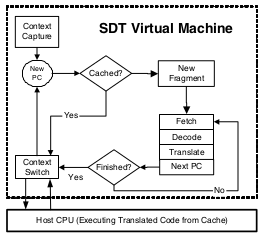
\includegraphics[scale=1]{Chapter3/Chapter3Figs/dynamic_algorithm.png} 
\caption{Dynamic translation algorithm}
\label{fig:dynamic translation algorithm}
\end{figure}

The task of the translation unit is to performs an application-specific translation and guarantee the correctness of the application. It starts fetching instructions from the address in the EIP register saved within the application context, until it reaches a  unconditional branch instruction or the maximum number of instruction per block.Than it decodes the instructions to be able to analyse them. It is particular interesting the approach taken by DynamoRio, which has developed an adaptive level-of-detail representation algorithm for decoding the instructions, where an instruction is only decoded and encoded as much as is needed. Note that there is not need to use a code discovery algorithm as in static approach because a fragment consists exclusively of instructions. Once the instructions are correctly translated,  they can be analysed for searching for instructions of interest. In the case of the system call interceptor the translation unit should search for instructions that might issue a system call request presented in \ref{binary_rewriting}. If one of those instructions is found, this must be overwritten with a jump to a system-call handling routine. Another advantage of performing binary rewriting at run time is that an instruction can always be substituted with another instruction even though the instruction set is of variable length. The translated instructions are copied in a new empty frame into the translation cache, therefore  there will always be enough space to allocate a jump instruction.   

During the translation process, the operand of a branch instruction must be adjusted to point to the translated block within the translation cache. This is ensue that only translated instruction are executed and therefore no system call invocation is missed. Usually the address are translated using a fast look-up hash table. 
If a translation for the target instruction does not exist, then the translation unit is invoked to translate the target block and insert it in the cache unit. Note that this approach might lead to duplicate code in the cache unit, for example when the operand of jump is an address pointing to an instruction in the middle of an block which has been already translated. A method used to improve the performance of handling branch instructions is to patch direct jumps and direct calls to avoid future lookups, this has been used in \cite{vx32, DynamoRio}. Unfortunately, patching cannot be used for indirect branches, including indirect calls and returns as their targets are variable. This hash table lookup for indirect branches, especially during return instructions, has been reported in \cite{vx32} to be the main source of slowdown in the execution of the dynamic rewritten binary. When the translation of a fragment is terminated, a context switch is performed and the application starts executing that fragment. The translation process is depicted in 


In the research literature, there are two examples of system call interceptor that are implemented following the approach previously discussed. The first is called Strata ,described in \cite{Strata}, where a system call interceptor has been used to ensure a safe virtual execution for an untrusted binary.  A 40\% of overhead is introduce in the execution of binary using the Strata tool, this is due principally to the rewriting process.  Strata has been implemented by following an easy approach concerning more about portability rather than performance and no optimizations have been introduced. A better and more complex example is implemented in vx32 \cite{vx32}. Vx32 is a lightweight sandbox that relies on segment protection as well as binary translation to confine an untrusted application.Vx32 is provided as static library that can be used to implement security tools. \emph{VxLinux} is a small system call interceptor implemented using vx32 library, it can be found at \cite{soft:vx32}. The interceptor mechanism is implemented following a delegating approach similar to that describe in chapter \ref{delegating_architecture}, it is able to run unmodified binary introducing an overhead spanning from 10\% to 50\% worst case. 


\section{Seccomp}
\label{seccomp}
A system call interceptor has been often employed in building sandboxing tools \cite{Janus, Garfinkel03ostia:a,MapBox, others}.The crucial aspect of these tools is security as a sandbox must guarantee that all system calls made by the sandboxed processes are correctly intercepted and verified. Current interposition-based mechanisms offer a wide variety of properties that make them an attractive approach for building sandboxing systems. Unfortunately, these are affects by numerous shortcomings that make their implementation difficult and a possible source of vulnerabilities. For instance, independently from the interceptor mechanism used, a sandbox has to deal with different type of race conditions such as arguments races, relative path races and symbolic link race, for a comprehensive list see \cite{garfinkel:traps, Watson_exploitingconcurrency}. These are sometimes referred to as \textit{Time of Check to Time of Use (TOCTOU)} races. In general, a race condition arises when there is a shared resource among different threads and the following actions occur : 
\begin{enumerate}

\item A sandbox grants permission to perform an operation A, that relies on some mutable shared state. For example, a shared buffer containing the name of a file is the arguments of a system call. 

\item Before the operating system starts performing the request, the shared resource is changed by another thread, making the operation A illegal. The sandbox will not intercept this action because a thread can modified a shared buffer without invoking a system call as the shared buffer is located in its own space memory. 

\item The operation A is performed by the operating system on the illegal values. 
\end{enumerate}  

This type of race condition is a significant problem for sandboxing tools and can be used to mislead introduction detections system and perform not authorized operations. In order to tackle these problems and simplify the implementation of sandboxing tools, a simple sandboxing mechanism called \textbf{seccomp} (short for secure computing mode)  has been introduced in Linux kernel 2.6.12. Seccomp isolates the execution of an untrusted process in its own address space by limiting the available system calls that the untrusted process can invoke. Seccomp mode can be enabled via the \ci{prctl} \cite{prctl}  system call using \ci{PR_SET_SECCOMP}  as first argument, when the system call returns,  the caller process enters seccomp mode. Seccomp has two different working modalities that can be selected via its second arguments:  

\begin{description}
\item[SECCOMP\_MODE\_STRICT] sets the most restrictive working mode where the only system calls that the thread is permitted to make are read, write, exit, an 
						sigreturn.  Other system calls result in the delivery of a SIGKILL signal that terminates the application's execution. Strict secure computing mode is
						useful for applications that may need to execute untrusted byte code obtained from an external source, for example, by	reading from a pipe or socket.
						Seccomp was first devised by Andrea Arcangeli in January 2005 for safely running numerical applications in public grid computing. It has also been
						used by Google to build a sandbox environment within Chrome called \textit{seccompsandbox} \cite{seccompsandbox}. This is used to restrict the execution
						of Adobe Flash Player and video renderers.
						
\item[SECCOMP\_MODE\_FILTER] has been recently introduced in Linux 3.5. This approach provides more flexibility respect the strict mode as it allows to define which system call
						should be denied via a Berkeley Packet Filter \cite{bpf} passed as third argument.This can be designed to filter arbitrary system calls and system call
						arguments. This approach has been used to implement \textit{minijail}  \cite{minijail} an new sandbox used in Chrome and in VSFTP \cite{vsftp}. 

\end{description}

In the remainder of this section the two seccom modes are analysed in better details. The  section \ref{seccompsandbox} introduces \textit{seccompsandbox}, the sandbox implemented in Chromium which uses a selective dynamic binary rewriting approach to implement a delegating system call interposition. While \ref{filter} present the features provided by the filtering mode of seccomp. 

\subsection{Seccomp mode strict}
\label{seccompsandbox}


Creating a sandbox in which to run untrusted code is a difficult problem. The successful sandbox implementations tend to come with completely new languages (e.g. Java) that are specifically designed to support that functionality. Try to sandbox an application at system call level as in Janus \cite{ Janus}, Ostia \cite{Garfinkel03ostia:a} is a much more difficult task due principally to the problems discussed in the previous section.
Seccomp offers a perfect solution for implementing a sandbox because it reduces the kernel attack surface to just four system calls. This ensures that, even though the application is compromise, an attacker cannot perform any permanent damage in the system. The only system calls allowed in seccom strict mode are : 
\begin{itemize}
\item  read/write can be used to write to or read from a file descriptor. Note that the file descriptor must be already open. 
\item  sigreturn is necessary to support correctly signal in Linux. This system call is called every time the signal handler has completed its task in order to return the control 	   to the original process. 
\item  exit	is used to terminate the process. 
\end{itemize}

If a process attempts to call any other system call, the entire process is terminated. This behaviour is very desirable from a security point of view, as it means that any failure in the sandbox causes the termination of the sandboxed process preventing possible unsafe actions.Seccomp was originally designed to isolate number-crunching applications in grid computing. Numerical applications usually do not require a large amount of system calls and thus they can be successfully executed just with these few system calls. However, this is not true in general; the four system calls allowed by seccomp are insufficient for most applications to run successfully. 

To overcome this limitation both \emph{seccompsandbox} and \emph{seccomp-nurse} run a trusted helper thread that does not enable seccomp. The helper thread opens a communication channel with the untrusted thread (e.g. using a socketpair or pipe). Now, any time the sandboxed thread wants to make a system call other than one of the four unrestricted system calls, it serializes the request and writes it over the communication channel with the helper thread.The helper then inspects the request and if it is a valid request, it executes it  on behalf of the sandboxed thread.This architecture has been depicted in Figure \ref{fig:seccomp}. 

\begin{figure}[b]
\centering
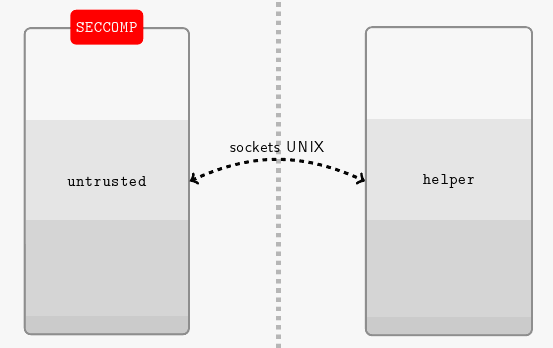
\includegraphics[scale=0.5]{Chapter3/Chapter3Figs/seccomp.png} 
\caption{Seccomp delegating architecture}
\label{fig:seccomp}
\end{figure}


This delegating architecture works for correctly most system calls, but a small number of system calls that manipulate the thread state need to be emulated differently. Notable and relevant examples are thread-local storage, and POSIX signals. Fortunately, TLS is a non-issue as it gets set up once at thread creation and is then not touched any more.Signals are more difficult and they are emulated in user-space. For an application that makes heavy use of signals, this could turn out to be a problem.

One of the requirement of a sandbox is to run untrusted binaries without requiring sources modifications and recompilation. In order to satisfy this requirement the delegating architecture presented so far must solve two problems. 
\begin{itemize}
\item  The first is how to insert the untrusted application in seccomp mode. The request to enter seccomp mode must be issued by the untrusted application, but none application 		   has been natively designed to work on seccomp mode.
\item The second problem is how to prevent the untrusted process from issuing system calls. All system call requests should be intercepted and routed to the helper thread before 		  the operating system start processing them, otherwise the application will be terminated. 
\end{itemize}

In order to insert the untrusted application in seccomp, a prtcl request must be inject into the untrusted application before its execution starts. This can be accomplished in different ways, for example by tracing the untrusted process and substituting its first system call request with a prctl request. While, seccompsandbox and seccomp-nurse use an approach based on LD\_PRELOAD\footnote{LD\_PRELOAD is a environment variable that contains a location of a shared object. During the linking phase this object will be linked to the binary allowing for symbols to be overwritten.} feature to solve this problem. 


The entry point of an executable file is the \emph{\_start} routine provided by the compiler. The main task of this routine is to initialize the stack and call the \lstinline$__libc_start_main$  provided by the GNU libc. The \lstinline$__libc_start_main$ routine performs some initialisation actions to set up the execution environment and then runs the application by calling its main function. The LD\_PRELOAD feature can be used to override the \lstinline$__libc_start_main$ function in order to call an arbitrary function. Seccomp-nurse uses this mechanism to initialize the sandbox environment and inject the prtcl request. The \lstinline$__libc_start_main$ is overridden by the function presented in Listing \ref{preload} during the load phase. This function retrieves the address of the original \lstinline$__libc_start_main$ function from the GUN libc library (lines) and then calls it by replacing the original main by a modified version called \lstinline$wrap_main$. This causes the execution environment to be properly initialised and the wrapper function to be executed. The aim of this wrapper function is to perform all those essential actions to correctly set up the sandbox environment, for example installing the communication channel with the helper thread. Once the initialisation phase is completed, a prctl request is issued and the application enters strict seccomp mode execution.  

\begin{center}
\label{preload}
\begin{lstlisting}[caption={Wrapper \_\_libc\_start\_main used in seccomp-nurse}]
typedef int (*main_t)(int, char **, char **);
main_t realmain;

int __libc_start_main(main_t main,
                      int argc,
                      char *__unbounded *__unbounded ubp_av,
                      ElfW(auxv_t) *__unbounded auxvec,
                      __typeof (main) init,
                      void (*fini) (void),
                      void (*rtld_fini) (void), void *__unbounded
                      stack_end)
{
        void *libc;
        int (*libc_start_main)(main_t main,
                               int,
                               char *__unbounded *__unbounded,
                               ElfW(auxv_t) *,
                               __typeof (main),
                               void (*fini) (void),
                               void (*rtld_fini) (void),
                               void *__unbounded stack_end);

        libc = dlopen("libc.so.6", RTLD_LOCAL  | RTLD_LAZY);
        if (!libc)
                ERROR("  dlopen() failed: %s\n", dlerror());
        libc_start_main = dlsym(libc, "__libc_start_main");
        if (!libc_start_main)
                ERROR("     Failed: %s\n", dlerror());

        realmain = main;
        return (*libc_start_main)(wrap_main, argc, ubp_av, auxvec,
        init, fini, rtld_fini, stack_end);
        
 		int wrap_main(int argc, char **argv, char **environ)
{
		if (socketpair(AF_UNIX, SOCK_STREAM, 0, fds) < 0) {
			    perror("socketpair failed");
                exit(1);
		
		}

        if (prctl(PR_SET_SECCOMP, 1, 0, 0) == -1) {
                perror("prctl(PR_SET_SECCOMP) failed");
                printf("Maybe you don't have the CONFIG_SECCOMP support built into your kernel?\n");
                exit(1);
        }

        (*realmain)(argc, argv, environ);
}       
}
\end{lstlisting}
\end{center}

Note that this method is affected by a serious vulnerability. A binary file can be generate in such way that the \emph{\_start} routine does not call the \lstinline$__libc_start_main$. In that case, the prtcl routine would not be called and the program would not run in a sandboxed environment. Seccompsandbox uses a similar approach, it loads am initialization function in memory using LD\_PRELOAD but it redirect the execution to this function using ptrace (i.e. it explicitly sets the pointer register to the entry within the object load via LD\_PRELOAD). This approach avoids the vulnerability previously discussed.  

Once the untrusted process has entered seccomp mode process, its attempts to invoke a system call must be intercepted before the operating system starts processing them and redirect to the helper thread. The helper thread then can thoroughly verify the system call and its arguments and decide whether execute or deny it. Seccompsandbox  uses a selective dynamic rewriter to intercept system call invocations made by the untrusted thread and the libraries to which it has been linked, this process is usually referred to as patching phase. The patching phase occurs during the initialization phase before the application enters seccomp mode. 

Seccompsandbox uses the rewriting method presented in BIRD \cite{BIRD} in a dynamic manner. The first difference between seccompsandbox and the binary methods previously discussed is that seccombsandbox reduces the discovery code phase to merely disassembling the application code segment. This implementation choice has been taken because it does not compromise the security of the sandbox as any failure to find the system call sites or any failure to correctly rewrite them would result in the termination of the application. 

System call instructions are rewritten with an unconditional jump instruction.  During the rewriting process, some instructions nearby the system call instruction may be relocate to provide enough space to locate the jump instruction. The target of the jump instruction is a routine that is dynamically allocated during the rewriting process via memmap system call. This routine accomplishes the following tasks in order to ensure that the application's behaviour has not been changed during the rewriting process :

\begin{itemize}
\item Executes the instructions that have been relocated during the rewriting process by guaranteeing the original order. Usually these instructions are referred to as preamble 		  and postable. 
\item Performs a translation between the system call convention (system call arguments within the registers) to the C function convention (functions arguments in the stack)   	  		  and call a dispatch routine which routes the system call invocation to the correct system call handler. 
\item Ensures that the rewriting process is fully transparent to the untrusted thread. This accomplished by saving the state before calling the dispatcher routine ans restoring 
	  it with the exception of the register that contains the result of the system call. 
\end{itemize}

Once the patching phase is completed, the system call requests are routed to the helper thread using the communication channel installed during the initialisation phase. This method and more in general a delegating architecture, requires to implement a dedicate handler for almost all system calls implemented in Linux. This is not a trivial implementation effort due principally to the high number of system calls (over 300) and their complexity. Some system calls, for example signal handling,memory mapping and process management, cannot be just executed on behalf of the untrusted thread as these system call may change the thread state.
The approach followed to address this problem usually consist of emulating kernel functionalities  at user space. However, in some case this is not possible as in the case of the clone system call and mmap. This is  one of the the main reason that has driven to develop an alternative solution.   

An exemple of this routine for x86\_32 architecture is presented in . 

\begin{lstlisting} 
	
	execute_preable()
	salve_state(); 
	// transform system call invocation to the c convention	
 	push %edi
    push %esi
    push %edx
    push %ecx
    push %ebx
    push %eax
    
    // Call default handler.
 	"call playground$defaultSystemCallHandler@PLT\n"
 	//clean the stack
 	"add  $24, %esp\n"
    restore_state(); 
    execute_
//

\end{lstlisting}


%%%%%%%%%%%%%%%%%%%%%%%%%%%%%%%%%%%%%%%%%%%%%%%%%%%%%%%%%%%%%%%%%%%%%%% SECCOMP BPF %%%%%%%%%%%%%%%%%%%%%%%%%%%%%%%%%%%%%%%%%%%%%%%%%%%%%%%%%%%%%%%%%%%%%%%%%%%%%%
\subsection{Seccomp mode filter}
\label{filter}
           

System call filtering architectures have been attempted many times \cite{Provos02improvinghost,Janus,MapBox, Noordende_asecure, Jain99user-levelinfrastructure}, but none of them has been capable to successfully address all problems correlated to race conditions discussed in\ref{seccomp}. Seccomp mode filtering is a promising technology that has been recently introduce in the Linux kernel (version 3.5) in order to provide a means of filtering the system call made by a program. Seccomp BPF is not a sandbox, but it  has been designed principally to be used by sandbox developers as it provides a clearly defined mechanism for minimizing the exposed kernel surface to user space. 

The filter capabilities are expressed through a Berkeley Packet Filter (BPF) program \cite{bpf}. When a program is in a seccomp mode, each system call request is  turned into a specific data structure so that, it can be processed by the BPF machine within the kernel. The fact the machine resides within the kernel provides a solution for time-of-check-time-of-use (TOCTOU) attacks that are common in system call interposition frameworks. Once the data has been fetched by the BPF machine and thus it resides in kernel space, it cannot be changed by any other thread in user space. However, this also implies some constrains in writing BPF filters. Most notably, a BPF program can't have loops, which bounds their execution time by a function of their size. Another advantages of this approach respect those analysed in the previous chapters is that the seccomp filter mode is automatically inherited by the children process created by the application via \ci{clone} or \ci{fork} system calls.

Seccomp filtering mode can be enabled by issuing the following request : 

\begin{center}
\lstset{escapechar=@,style=c}
\begin{lstlisting}[caption={Request for entering seccomp filtering mode}]
												prctl(PR_SET_SECCOMP, SECCOMP_MODE_FILTER, bpf_filter);
\end{lstlisting}
\end{center}

The \ci{bpf_filter} argument is a pointer to a struct \ci{sock_fprog} which contain the filter program.  If the program is invalid, the call will fail. The BPF program will be executed over struct \ci{seccomp_data} reflecting the system call number, arguments, and other metadata necessary to correctly analyse it. Once the program has entered seccomp filtering mode, each time it makes a system call, the BPF filter program is executed in order to verify whether the system call should be executed or not. The execution of the filter may introduce a significant overhead on the application's execution, therefore the BPF program should be as shorter as possible to reduce this overhead. The BPF program must return a values to inform the kernel which action should be taken. A seccomp filter supports many different returning values, we focus only on those interesting for implementing a system call interceptor, for an complete list see \cite{filtering}.  

\begin{description}
\item[SECCOMP\_RET\_KILL]  Results in the task exiting immediately without executing the system call. 
\item[SECCOMP\_RET\_ALLOW] Results in the system call being executed.
\item[SECCOMP\_RET\_TRAP]  Results in the kernel sending a \ci{SIGSYS} signal to the triggering task without executing the system call. 
\item[SECCOMP\_RET\_TRACE] Results in the kernel to attempt to notify a ptrace-based tracer the system call request prior to executing it.  If there is no tracer present,
						   \ci{ENOSYS} is returned to user space and the system call is not executed.
\end{description}

The BPF machine consists of an accumulator, an index register, a scratch memory store, and an implicit program counter.BPF filtering programs are expressed in pseudo assembler instructions. Each instruction consists of an OPCODE field that defines the instruction itself and tree additional arguments whose meaning depends on the value specified on the OPCODE field.  Programs expressed in BPF filtering language  are rather flexible, they can fetch data, perform arithmetic operations, and perform tests, and notify to the kernel whether an event (e.g. a system call) should be accepted or not via the return value. A full description of the BPF machine and its assembler language can be found in \cite{bpf}.

Linsting \ref{bpf_filter} presents how to use a BPF filter within seccomp filtering mode for intercepting a system call. The task accomplished by this program is quite simple, it merely checks that a program uses the write system call only for writing to the standard output. A BPF program must begin by checking the underlying architecture in order to verify whether it can be run correctly. This is necessary because some architecture may use a different system call convention and therefore the filter is not applicable (for example, a filter written for x86\_32 is not portable on x64). Once the safety checks have been completed, the first operation is issued. The system call number is loaded into the accumulator register using the store instruction \ci{BPF_SRMT}. Then, the system call can be identified using a \ci{BPF_JUMP} instruction which compares the value within the accumulator register with a constant and jumps to the offset specified as second argument is the result is positive or to the third argument if the result is negative. If the system call invoked is not a write, the execution is redirected  to the last instruction which allows the system call. While if the system call requested is write, the first system call argument is retrieved using the macro \ci{LO_ARG}\footnote{\ci{LO_ARG} is a macro defined as follows : \\
\ci{#define LO_ARG(idx) offsetof(struct seccomp_data, args[(idx)])}.
}.The first argument contains the file descriptor used by the write system call.  The filter verifies if this descriptor is the standard output in a similar manner as the previous case. If an attempt of writing to a different file descriptor is found the system call is denied and the entire process in terminated. While, if the argument is correct the execution continues.   

\begin{center}
\lstset{escapechar=@,style=c_num}
\begin{lstlisting}[label=bpf_filter,caption={BPF filter ensuring that a program can write only over the standard output}]
		/* Validate Architecture */
		BPF_STMT(BPF_LD+BPF_W+BPF_ABS, arch_nr), 
		BPF_JUMP(BPF_JMP+BPF_JEQ+BPF_K, ARCH_NR, 1, 0), 
		BPF_STMT(BPF_RET+BPF_K, SECCOMP_RET_KILL), 
		
		/* Load system call number in the accumulator */
		BPF_STMT(BPF_LD+BPF_W+BPF_ABS, syscall_nr),
		/* Check if the system call is read */
		BPF_JUMP(BPF_JMP+BPF_JEQ+BPF_K, __NR_write, 0, 4),
		/* Access to its first argument */
		BPF_STMT(BPF_LD+BPF_W+BPF_ABS, LO_ARG(0)),
		/* Verify that the file descriptor points to STDIN */
		BPF_JUMP(BPF_JMP+BPF_JEQ+BPF_K, STDOUT_FILENO, 1, 0),
		/* The system call is denied */
		BPF_STMT(BPF_RET+BPF_K, SECCOMP_RET_KILL),
		/* The system call is allowed */
		BPF_STMT(BPF_RET+BPF_K, SECCOMP_RET_ALLOW),

\end{lstlisting}
\end{center}

The definition of BPF filters is a bit cumbersome due to low expressiveness and readability of BPF assembly instructions. The appendix B presents a C header file containing some  macros that simplify the definition of BPF filter by providing the basic functionalities (e.g. deny or allow a system call) as an extra instruction (e.g. for allowing the system call name, \ci{ALLOW_SYSCALL(name)}). In addition, this increases the readability of the code as each macro is defined with a name that specifies its task. 

The introduction of seccomp-bpf in the kernel has also provided a new way to trace the execution of a process via ptrace. The seccomp-bpf filter can turn system call into tracer event by returning \ci{SECCOMP_RET_TRACE}. The tracer process must specify the option \ci{PTRACE_O_TRACESECCOMP} for receive the seccomp notification  and then it will be notified of seccomp events \ci{PTRACE_EVENT_SECCOMP}. Instead of using the \ci{PTRACE_SYSCALL} to resume the execution of the tracee, the tracer can use \ci{PTRACE_CONT} to only listen for events.

This new method improve and solve some problems affecting the standard ptrace tracing mechanism. First of all, it allows to selectively intercept system calls by setting the trace option in the filter only for a subset of system calls, while allowing the execution of the others. The first consequence of this is that the overall performance will increase as the tracing overhead is reduced to only the system call of interest. 

%The second major benefit introduced by this method is that, it provides a valid solution for tracing multithread applications. BPF-filters are inherited by all new processes spawned by a process in seccomp mode, therefore there is not need to att   

Seccomp filter represent a valid and interesting solution for developing sandboxes. In  fact, it has been already employed to increase the security of two important software. The first is \emph{minijail} \cite{minijail}, the new sandbox realized by Google in order to increase the security of Chrome. The second is VSTP \cite{vsftp} a secure FTP daemon largely used. However, the sandbox is not the only possible use of seccomp-bpf. The User Mode Linux project has expressed interest in seccomp-bpf, especially for the trap functionality which would allow them to emulate a system call without using ptrace. Finally another project that is worth mentioning, is a new library called \emph{libseccomp} \cite{libseccomp} that has been developed to ease the definition of BPF filter for a seccomp application.   
